% ----------- Cover Master Thesis Faculty of Sciences ---------------
% This document should be compiled with pdflatex.  If you want to use
% latex to compile to dvi/ps, you have to convert the images to (e)ps
%                           -- December 2012
% -------------------------------------------------------------------
\RequirePackage{fix-cm}
\documentclass[12pt,a4paper,oneside]{book}

% ------------------------- Load packages ---------------------------
% You can eventually add these while you load other packages
% in case you want to integrate the titlepage with the rest of your thesis
% -------------------------------------------------------------------
\usepackage{graphicx,xcolor,textpos}
\usepackage{helvet}
\renewcommand{\familydefault}{\sfdefault}
\usepackage{amsmath, amsfonts, amssymb, amsthm}
\usepackage{tikz}
\usepackage{url}
\usepackage{hyperref, cleveref}
\usepackage{subcaption}
\usepackage{chngcntr}
\usepackage{quiver}
\usepackage{biblatex}
\addbibresource{thesis_references.bib}
% ------------------------ Page settings -----------------------------
% If you change these, the cover layout will also change.  In that
% case you have to adjust the latter manually.
% --------------------------------------------------------------------

\topmargin -10mm
\textwidth 160truemm
\textheight 240truemm
\oddsidemargin 0mm
\evensidemargin 0mm

% ---------------------- textpos settings ----------------------------
% Some additional settings for the cover
% --------------------------------------------------------------------

\definecolor{bluetitle}{RGB}{29,141,176}
\definecolor{blueaff}{RGB}{0,0,128}
\definecolor{blueline}{RGB}{82,189,236}
\setlength{\TPHorizModule}{1mm}
\setlength{\TPVertModule}{1mm}

% --------------------------- Other Definitions ------------------------
% Additional definitions for particular environments
% ----------------------------------------------------------------------

\def\reals{\mathbb{R}} %real numbers
\def\complex{\mathbb{C}} %complex numbers
\def\naturals{\mathbb{N}} %natural numbers
\def\integer{\mathbb{Z}} %integers
\def\proj{\mathbb{P}} %Projective
\def\aff{\mathbb{A}} %Affine
\def\var{\mathbb{V}} %Variety
\def\ideal{\mathbb{I}} %Ideal
\def\field{\mathbb{F}} % Field
\def\rank{\text{Rank}} % Rank
\def\srank{\text{Rank}_S} % Symmetric Rank
\def\borderrank{\underbar{\rank}} %Border Rank


\newtheorem{theorem}{Theorem}[section]
\newtheorem{conjecture}{Conjecture}
\newtheorem{lemma}[theorem]{Lemma}
\newtheorem{corollary}{Corollary}[theorem]
\newtheorem{proposition}{Proposition}[section]

\theoremstyle{definition}
\newtheorem{definition}{Definition}[section]
\newtheorem*{example}{Example}
\newtheorem*{observation}{Observation}
\newtheorem*{remark}{Remark}

\hypersetup{
    colorlinks=true,
    linkcolor=red,
}

\counterwithout{figure}{chapter}
\begin{document}

% ----------------------- Cover --------------------------------------
% Please fill in:
% - The title and subtitle (if applicable)
%         to include a formula in the title or subtitle
%         use  \form{$...$}
% - Your name
% - Your (co)supervisor, mentor (if applicable)
% - Your master
% - The academic year
% --------------------------------------------------------------------
\thispagestyle{empty}
\newcommand{\form}[1]{\scalebox{1.087}{\boldmath{#1}}}
\sffamily
%
\begin{textblock}{191}(-24,-11)
\colorbox{bluetitle}{\hspace{139mm}\ \parbox[c][18truemm]{52mm}{\textcolor{white}{FACULTY OF SCIENCE}}}
\end{textblock}
%
\begin{textblock}{70}(-18,-19)
\textblockcolour{}
\includegraphics*[height=19.8truemm]{LogoKULeuven}
\end{textblock}
%
\begin{textblock}{160}(-6,63)
\textblockcolour{}
\vspace{-\parskip}
\flushleft
\fontsize{40}{42}\selectfont \textcolor{bluetitle}{The State of Comon's Conjecture 
% \form{$a^2+b^2=c^2$}
}\\[1.5mm]
% \fontsize{20}{22}\selectfont Subtitle \form{$S=\pi r^2$\textsl{(optional)}}
\end{textblock}
%
\begin{textblock}{82}(50,103)
\textblockcolour{}
\vspace{-\parskip}
\flushleft
% \fbox{\parbox{79mm}{The background can be left blank or you can insert an image (maximum height 10 cm, width variable, mind author’s rights…). NO logos (you can use the logos inside the manuscript, but not on front or back cover). \textit{Delete this textbox.}}}
\end{textblock}
%
\begin{textblock}{160}(8,153)
\textblockcolour{}
\vspace{-\parskip}
\flushright
\fontsize{14}{16}\selectfont \textbf{Lael JOHN}
\end{textblock}
%
\begin{textblock}{70}(-6,191)
\textblockcolour{}
\vspace{-\parskip}
\flushleft
Supervisor: Prof. N. Vannieuwenhoven\\[-2pt]
\textcolor{blueaff}{KU Leuven}\\[5pt]
Co-supervisor: Dr. D. Taufer\\[-2pt]
\textcolor{blueaff}{KU Leuven}\\[5pt]
% Mentor: Dr. D. Taufer\\[-2pt]
% \textcolor{blueaff}{KU Leuven}\\
\end{textblock}
%
\begin{textblock}{160}(8,191)
\textblockcolour{}
\vspace{-\parskip}
\flushright
Thesis presented in\\[4.5pt]
fulfillment of the requirements\\[4.5pt]
for the degree of Master of Science\\[4.5pt]
in Mathematics\\
\end{textblock}
%
\begin{textblock}{160}(8,232)
\textblockcolour{}
\vspace{-\parskip}
\flushright
Academic year 2025 -2026
\end{textblock}
%
\begin{textblock}{191}(-24,248)
{\color{blueline}\rule{550pt}{5.5pt}}
\end{textblock}
%
\vfill
\newpage

% In case you want to integrate the TeX-file for the titlepage
% with the rest of your thesis, you cab continue below
% ------------------------- First pages ---------------------------
% For table of contents, acknowlegments, ...
% -----------------------------------------------------------------
\sffamily
\setcounter{page}{0}
\pagenumbering{roman}

\tableofcontents
\listoffigures
\newpage
% -------------------------- Proper text --------------------------
% Introduction, chapters, ...
% -----------------------------------------------------------------
\setcounter{page}{0}
\pagenumbering{arabic}

\chapter*{Introduction}
The topic of this thesis centers around an open question about tensors. These are mathematical tools, used to describe relationships between multiple objects, allowing for some form of algebra to occur. In context of this work, the focus remains on how tensors can be built, where they lie, and how they can be broken down. 

The state of Comon's conjecture (an open problem for the last 20 years) is not easily described. While mathematicians have chipped away at the number of cases where it remains valid, an answer in full generality over $\reals$ or $\complex$ remains unknown. The hope is that at least some of the work done in recent years can be highlighted as useful, paving the way towards a definitive counterexample or proof.
\begin{figure}
    \centering
    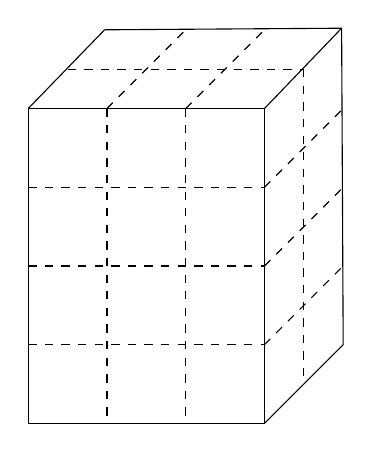
\begin{tikzpicture}[scale=1]
        % Coordinates
        \coordinate (A) at (1.00, 8.00);
        \coordinate (B) at (1.97, 9.00);
        \coordinate (C) at (4.00, 8.00);
        \coordinate (D) at (4.98, 9.02);
        \coordinate (E) at (4.00, 4.00);
        \coordinate (F) at (5.00, 5.00);
        \coordinate (G) at (1.50, 8.50);
        \coordinate (H) at (4.50, 8.50);
        \coordinate (I) at (4.50, 4.50);
        \coordinate (J) at (2.00, 8.00);
        \coordinate (K) at (2.00, 4.00);
        \coordinate (L) at (3.00, 8.00);
        \coordinate (M) at (3.00, 4.00);
        \coordinate (N) at (3.00, 9.00);
        \coordinate (O) at (4.00, 9.00);
        \coordinate (P) at (1.00, 7.00);
        \coordinate (Q) at (4.00, 7.00);
        \coordinate (R) at (5.00, 8.00);
        \coordinate (S) at (1.00, 6.00);
        \coordinate (T) at (4.00, 6.00);
        \coordinate (U) at (5.00, 7.00);
        \coordinate (V) at (1.00, 5.00);
        \coordinate (W) at (4.00, 5.00);
        \coordinate (X) at (5.00, 6.00);

        % Drawing
        \draw (1,4) rectangle (4,8);
        \draw (A) -- (B);
        \draw (C) -- (D);
        \draw (E) -- (F);
        \draw (B) -- (D);
        \draw (F) -- (D);
        \draw[dashed] (G) -- (H);
        \draw[dashed] (H) -- (I);
        \draw[dashed] (J) -- (K);
        \draw[dashed] (L) -- (M);
        \draw[dashed] (J) -- (N);
        \draw[dashed] (L) -- (O);
        \draw[dashed] (P) -- (Q);
        \draw[dashed] (Q) -- (R);
        \draw[dashed] (S) -- (T);
        \draw[dashed] (T) -- (U);
        \draw[dashed] (V) -- (W);
        \draw[dashed] (W) -- (X);
        \end{tikzpicture}
    \caption{Example of a tensor $T \in \field^4 \otimes \field^3 \otimes \field^2$}
\end{figure}
This question merits study because of the powerful nature of tensors as descriptors of relationships. Tensors find their use in quantum mechanics, general relativity \cite{carroll_spacetime_2019}, chemometrics, psychometrics\cite{zhang_comons_2016}, and signal processing \cite{landsberg_tensors_2012} --- to name some examples. In each of these cases, knowing how important a feature of the relationship symmetry is would play a vital role in analysing procedures and algorithms that take for granted that symmetry is the more "natural" state of affairs. This forms the guiding idea behind the ideas and techniques explored during this thesis.

\section*{Comon's Conjecture}\label{section:comonsconjecture}
At its heart, Comon's Conjecture centers around 2 central themes: rank and symmetry in tensors. Rank (see \cref{defn:tensorrank}) describes how a tensor can be decomposed into simpler constituent tensors, and symmetry (see \cref{defn:symmetrictensor}) describes how tensors behave under permutation actions.

The conjecture was first stated openly in July 2008 at "Geometry and Representation Theory of Tensors for Computer Science, Statistics and Other Areas" - a workshop organised at the American Institute for Mathematics \cite{oeding_report_2008} in the group focusing on "Multilinear Techniques in Data Analysis and Signal Processing". The conjecture as stated in the report is as follows

\begin{conjecture}[Comon]
    Do the rank and symmetric rank of $T$ always coincide, where $T$ is a real or complex tensor?
\end{conjecture}

The report also covered work done previously by Comon et al. \cite{comon_symmetric_2008} where they also showed that the conjecture held for situations when the symmetric rank was at least as large as the dimension, or when the order (see \cref{defn:tensororder}) of $T$ is sufficiently large. Since 2008, the mathematical community has proved the conjecture true under various assumptions (see \cref{section:pastoverview}). 

In 2019, Shitov \cite{shitov_counterexample_2018} proposed the construction of a counterexample living in $(\complex^{800})^{\otimes 3}$ with symmetric rank at least $904$, and a rank of at most $903$. In 2024 however, an erratum published \cite{draisma_erratum_2024} showed a flaw in the construction, rendering the conjecture still open, at least for the complex case. In the intervening time, a paper published by Seigal and Wang \cite{wang_lower_2023} demonstrated the construction of a real, order $6$, symmetric tensor with real rank $30913$ and symmetric rank $30914$, disproving the conjecture for the real case. This paper built on constructions described in Shitov \cite{shitov_comons_2020}, a preprint, whose ideas have been developed further in subsequent preprints \cite{shitov_higher_2024} and \cite{shitov_higher_2024-1}.

The following chapters and sections highlight important terminology required to state and describe the setting of Comon's conjecture, highlight the work done to prove the conjecture in the past, and finally to describe the major constructions required to construct the real counterexample. 

\chapter{Preliminaries Regarding Tensors}\label{chapter:preliminaries}

%   FORMALLY DEFINE/HIGHLIGHT ORDER DEFINITION
\section{Tensors in an Algebraic Setting}\label{section:tensoralgebra}
The most abstract way of thinking about tensors is when describing them as elements of the tensor product of modules. Consider $A, B$ and $P$ as being $R$-modules, where $R$ is a ring. Then any mapping $t: A \times B \to P$ that is bi-linear in nature is described by acting on elements in this manner: $t(\lambda a, b) = t(a, \lambda b) = \lambda t(a, b)$, where $a \in A, b \in B, \lambda \in R$ and $t(a,b) \in P$ . 

\begin{figure}[h]
    % https://q.uiver.app/#q=WzAsMyxbMCwwLCJBIFxcdGltZXMgQiJdLFsyLDAsIlAiXSxbMSwxLCJBIFxcb3RpbWVzX1IgQiJdLFswLDEsImZcXDsgXFx0ZXh0e211bHRpbGluZWFyfSA9IFxcdGlsZGV7Zn0gXFxjaXJjIFxcdmFycGhpIl0sWzAsMiwiXFx2YXJwaGkiLDJdLFsyLDEsIlxcZXhpc3RzICFcXHRpbGRle2Z9IiwyXV0=
    \[\begin{tikzcd}
        {A \times B} && P \\
        & {A \otimes_R B}
        \arrow["{t\; \text{bilinear} = \tilde{t} \circ \varphi}", from=1-1, to=1-3]
        \arrow["\varphi"', from=1-1, to=2-2]
        \arrow["{\exists !\tilde{t}}"', from=2-2, to=1-3]
    \end{tikzcd}\]
    \caption{Illustrating the tensor product of $R$-modules}\label{fig:tensorcommutativediagram}
\end{figure}

Such a bilinear (or even multilinear mapping) between $R$-modules can be represented by an element lying in their tensor product, such that the following diagram of modules commutes \cite{vakil_rising_2025} (illustrated specifically for the case mentioned above in Figure \cref{fig:tensorcommutativediagram})

While such a description is useful when dealing with talking about how any general elements lying in spaces can be combined, this description lacks some of the necessary details required for actually computing what a tensor \textit{is}, or even how it can be represented.

A more useful approach to tensors is to begin from linear algebra. As matrices represent linear transformations between vector spaces $V$ and $W$, so $d$-way arrays can be used to represent multilinear relationships between vector spaces $V_1, V_2 \ldots V_d$. Diving deeper into this analogy, matrices do behave as either bilinear maps from the product $V \times W \to \mathbb{F}$, or as linear maps $W^* \to V^*$. This hybrid nature of matrices is in fact a reflection of the fact that matrices are order $2$ tensors. Since computing elements of the matrix $A_{ij}$ depends on a choice of bases for both vector spaces $V$ and $W$, an analogous choice of bases must be made to describe the order $d$ tensor $T \in V_1 \otimes V_2 \otimes \cdots \otimes V_d$. 

For the purposes of this thesis, unless specified, each vector space will be considered over $\field = \reals$ or $\complex$, with its standard ordered basis $\{e_i\}_{i=1}^{n}$ where $e_i(j) = \delta_{i,j}$. Accordingly, each vector space $V_i$ has a dimension $n_i$.
\begin{definition}[Order of a Tensor]\label{defn:tensororder}
    A tensor $T$ is said to be a $d$-order tensor, if $T \in V_1 \otimes \cdots\otimes V_d$.
\end{definition}
Let $T := v_1 \otimes \cdots \otimes v_d$ be an order-$d$ tensor, with each component $v_i \in V_i$ a vector with components $v_i(j)$ according to the standard ordered basis of the corresponding vector space. Then the elements of the $d$-way array that corresponds to $T$ can be given in the following manner $$T(k_1 | k_2 | \ldots | k_d) = \prod_{i=1}^{d} v_i(k_i)$$where $0 \leq k_i \leq n_i$--- the dimension of each corresponding vector space $V_i$.

$T$ as defined above can be seen in the following manner \begin{enumerate}
    \item as a multilinear mapping between $V_1^* \times V_2^* \times \cdots \times V_d^* \to \mathbb{F}$ (extending the analogue of looking at matrices as bilinear forms) $$(f_1, f_2 \ldots f_d) \mapsto \prod_{i=1}^{d} f_i(v_i)$$
    \item as a linear mapping from $V_i^* \to V_1 \otimes \cdots \otimes V_{i-1} \otimes V_{i+1} \otimes \cdots V_d =: V_{\hat{i}}$ (moving from a space of order-$d$ tensors to order-$d-1$) $$f_i \mapsto f_i(v_i)(v_1 \otimes \cdots \otimes v_{i-1}\otimes v_{i+1} \otimes \cdots \otimes v_d)$$
    \item as the dual of this previously defined linear map, now going from $V_{\hat{i}}^* \to V_i$ (moving now from order-$d$ to a vector collinear to $v_i$)$$(f_j)_{j \neq i} \mapsto \left(\prod_{j \neq i} f_j(v_j)\right)$$
\end{enumerate}

Each of these above viewpoints also corresponds to an appropriate transformation of the representative $d$-way array chosen, either to a scalar, $d-1$-way array or a vector respectively \cite{landsberg_tensors_2012}. In fact scalars and vectors now can also be seen as tensors of orders $0$ and $1$ respectively. 
\section{Tensors in a Geometric Setting}\label{section:tensorgeometry}
As with any textbook in linear algebra, working algebraically helps in terms of computation, but concepts rarely exist only algebraically. Matrices (and by extension tensors), physically describe how points can be transported from one space to another --- making them not just maps between algebraic structures, but also indicating a geometric nature. 

To start with, $2\times2$ matrices can be seen as points lying in the space $Mat(2, \mathbb{F})$, or as elements of $\mathbb{F}^4$. Adding further constraints to them: requiring the matrices to have a non-vanishing determinant, or a unit determinant, or even all entries as positive further allows us to look at these as points lying in $GL(2,\mathbb{F}), SL(2,\mathbb{F})$ or $Mat(2, \mathbb{F})_{\geq 0}$ respectively. Each of these examples correspond to a well studied geometric space.

Moving to the case of order-$d$ tensors, consider again a non-zero tensor $T:= v_1 \otimes \cdots \otimes v_d$. Because tensors are importantly multilinear as mappings, this means that none of the individual component vectors $v_i = 0$. Then for each individual $V_i$, the non-zero vector $v_i$ lies on a unique line through the origin $[v_i]$, allowing for a map between $V_i \to \proj V_i$, the projectivisation of $V_i$. Note here that when moving to the projectivisation, even though the number of coordinates we use to describe $v_i$ is $n_i$, the space $\proj V_i$ has dimension $n_i - 1$.

The component vectors of $T$ can now be written as a tuple lying in the Cartesian product of $d$ projective spaces i.e. $([v_1], \ldots, [v_d]) \in \proj V_1 \times \cdots \times \proj V_d$. A next natural question that arises is to see if such a tuple can be seen as lying in a much larger projective space, and this turns out to have an affirmative answer.
\begin{definition}[Segre Mapping]\label{defn:segremapping}
    Define $\Sigma: \proj V_1 \times \cdots \times \proj V_d \to \proj V$ as the following mapping $$([v_1], \ldots, [v_d]) \mapsto [v_1 \otimes \cdots \otimes v_d]$$The image point lies in the projectivisation of $V$, a vector space over $\field$ of dimension $\prod_{i=1}^{d} n_i$. Specifically all the image points lie in $\proj (V_1 \otimes \cdots \otimes V_d) \subseteq \proj V$ \cite{smith_invitation_2004}
\end{definition}
The existence of such a mapping allows for non-zero order-$d$ tensors (of the same form as \cref{defn:elementarytensors}) to be represented as points lying on this new \textit{Segre variety}.

\begin{lemma}
    The Segre mapping as defined above is an injective map, but not surjective.
\end{lemma}
\begin{proof}
    This mapping is well defined (all tuples have an image in $\proj V$, and the image of a tuple is unique). However, the Segre mapping is generally not surjective. Not every point in $\proj V$ can be written as the image of a single tuple of the form $([v_1], \ldots, [v_d])$. A simple example is when dealing with $3 \times 3$ matrices $[e_1 \otimes e_1 + e_2 \otimes e_2]$ cannot be written as the image of a single tuple of $([v_1], [v_2])$. 

    Starting with two distinct tuples $([a_1], \ldots, [a_d])$ and $([b_1], \ldots, [b_d])$ gives us at least one pair of vectors $a_i, b_i$ that do not lie on the same line through the origin in $V_i$. The resulting images under $\Sigma$ are the tensors $[a_1 \otimes \cdots \otimes a_d]$ and $[b_1 \otimes \cdots \otimes b_d]$ that differ at least in one component in the $d$-way arrays, and therefore represent distinct families of tensors. Thus the Segre mapping is injective, and ends up being referred to as the Segre \textit{embedding} in algebraic geometry litereature.
\end{proof}

%DOES IT MAKE SENSE TO DISCUSS THE GEOMETRIC IMAGES OF THE FLATTENINGS/SLICES?
\subsection*{Why is it important to consider both?}
Both aspects prove useful as tools to study tensors. Explicit computation is far easier when working with tensors algebraically, and thus much more easily applicable in fields other than mathematics, once problems have been stated in appropriate terms. On the other hand, dealing with the geometry of tensors allows for a much better examination of edge cases and boundary conditions, particularly useful when working with proofs about general properties that should apply to tensors. 
\section{Rank}\label{section:tensorrank}
While the previous two sections covered the nature of tensors, it is necessary to figure out how tensors can be constructed, since the Segre embedding example shows that there are tensors that cannot be constructed as simply the tensor product of vectors --- as an analogy, recall not all vectors in a vector space can be written as only scaled basis vectors.
\begin{definition}[Elementary Tensor]\label{defn:elementarytensors}
    Consider a tensor $T := v_1 \otimes \cdots \otimes v_d \in V_1 \otimes \cdots \otimes V_d$, an order $d$ tensor. Since $T$ can be written explicitly as the tensor product of $d$ vectors, it is known as an elementary tensor. Equivalent names for such tensors present in literature are \textit{rank one} and \textit{decomposable}.
\end{definition}
The Segre Variety (as defined in \cref{defn:segremapping}) contains exactly the images of all the non-zero \textit{elementary} tensors in a given tensor product. This still leaves open the question of how tensors of higher rank can be represented, which has been tackled successfully in the literature by the developement of \textit{secant varieties} \cite{bernardi_hitchhiker_2018} (see \cref{section:pastoverview})

Using these elementary tensors as building blocks now provides a way to describe the construction of more general tensors. 
\begin{definition}[Tensor Decomposition]\label{defn:decomposition}
    Consider a general tensor $T \in V_1 \otimes \cdots \otimes V_d$. A decomposition of $T$ consists of writing $T$ as a sum of elementary tensors $$T = \sum_{i=1}^{s} v_1^i \otimes \cdots \otimes v_d^i$$now with each of the $v_j^i \in V_i$. \cite{zhang_comons_2016}
\end{definition}
For any given tensor $T$ now, there can exist multiple decompositions, not just depending on the choice of basis vectors for each $V_i$. A further natural question to ask is if there is a shortest decomposition, and if such a decomposition is unique. 
\begin{definition}[Tensor Rank]\label{defn:tensorrank}
    The rank of a tensor $T$ is the minimal length of any possible decomposition of $T$.
\end{definition}
Tensor rank always exists, because tensors can always be written in terms of elementary tensors. Computing the rank of a given tensor is not an easy problem, but it has given rise to multiple approaches in the literature that rely on both the algebraic properties of tensors and associated transformations, and the geometric properties of the varieties on which these tensors lie. Tensor rank also remains invariant of decomposition and is one of the two key ingredients required to state Comon's Conjecture.

A further question that can be asked is whether "perturbing" a tensor changes its rank. This leads to the notion of describing rank when it is seen as the limit of a sequence. 
\begin{definition}[Border Rank]\label{defn:borderrank}
    A tensor $T$ has border rank $r$ if it can be expressed as a limit of a sequence of tensors of rank $r$, but not for any sequence of tensors with rank $s < r$. Conventional notation is to denote border rank with $\underbar{\rank}(T) = r$
\end{definition}
The notion of border rank comes in use when working with secant varieties, as a tool to help compute rank. Tensors can have differing ranks and border ranks
\begin{example} 
    Consider $T:= a_1 \otimes b_1 \otimes c_1 + a_1 \otimes b_1 \otimes c_2 + a_1 \otimes b_2 \otimes c_1 + a_2 \otimes b_1 \otimes c_2$ Then the rank of this tensor is 3, but one can write $T$ as the limit of tensors of rank 2 in the following manner $$T(s) = \frac{1}{s}\left((s-1)a_1 \otimes b_1 \otimes c_1 + (a_1 + sa_2)\otimes (b_1 + sb_2) \otimes (c_1 + sc_2)\right)$$ \cite{landsberg_tensors_2012}
\end{example} 


\section{Symmetric Tensors}\label{section:symmetrictensors}
The other half of Comon's Conjecture revolves around tensors that exhibit symmetric properties. These become valuable in applications simply because the symmetry means that they require "less" information to be constructed. What makes a tensor symmetric is the next logical question to tackle, and necessitates a definition of how permutations act on a given tensor.

Given $\sigma \in S_d$, an element representing a permutation of $d$ distinct elements, then one can define the permutation action on a tensor as follows
\begin{definition}[Permutation of a Tensor]\label{defn:tensorpermutation}
    Let $T:= v_1 \otimes \cdots \otimes v_d \in V_1 \otimes \cdots \otimes V_d$, where $V_i = V_j$. Then $\sigma \in S_d$ acts on $T$ in the following manner $$\sigma \cdot T = v_{\sigma(1)} \otimes \cdots \otimes v_{\sigma(d)}$$
\end{definition}
Note here that we do require that all the vector spaces are the same, to keep the mapping well defined. If the vector spaces were allowed to differ in dimension, then this would no longer be a group action, since the underlying set keeps changing (shuffling around.) This also allows for the use of notation $T \in V^{\otimes d}$. Such tensors are also referred to as \textit{cubical}.

The definition of a symmetric tensor follows almost immediately 
\begin{definition}[Symmetric Tensor]\label{defn:symmetrictensor}
    Consider a tensor $T \in V^{\otimes d}$. $T$ is said to be symmetric if the following equality holds $$T = \frac{1}{d!} \sum_{\sigma \in S_d} \sigma \cdot T$$The requirement of $T = \sigma \cdot T$ for all $\sigma \in S_d$ follows as a consequence of this definition. \cite{comon_symmetric_2008}.
\end{definition}

Further, since very tensor can be expressed as a decomposition (see \cref{defn:decomposition}), it follows that symmetric tensors can also be decomposed into a sum of elementary \textit{symmetric tensors}, where now each is of the form $v^{\otimes d}$ by symmetry requirements.

It is clear that not every tensor can be seen as symmetric, and therefore the subset of all order $d$ tensors that are symmetric is denoted $S^d(\field^n) \subseteq \field^n$ --- notation usually reserved for homogenous polynomials in $n$ variables of fixed degree $d$. In fact one can show that these spaces are isomorphic to each other. This equivalence is a powerful tool that allows for an interchange of polynomial and tensor notation (when appropriate).

\subsection*{Symmetric Tensors and Homogenous Polynomials of Fixed Degree}\label{subsection:homogenouspolyrelation}
A polynomial $f \in \field[x_1, \ldots, x_n]_d$ is of the form $$f(x_1, \ldots x_n) = \sum_{a_i \geq 0, \sum_{i}^{n} a_i = d} \lambda_{(a_1, \ldots, a_n)}\prod_{i=1}^{n}x_i^{a_i}$$where all the coefficients $\lambda_{(a_1, \ldots, a_n)} \in \field$. Here the following notation is commonly used in the literature --- $\mathbf{x} = (x_1, x_2, \ldots x_n)$ and $\mathbf{\alpha} = (a_1, a_2, \ldots a_n) \in (\naturals \cup \{0\})^n$. Then $\mathbf{x^{\alpha}} = \prod_{i=1}^{n}x_i^{a_i}$. Further $|\mathbf{\alpha}| = \sum_{i}^{n} a_i$, so the homogenous polynomial as stated above can be rewritten as $$f(\mathbf{x}) = \sum_{|\mathbf{\alpha}| = d} \lambda_{\mathbf{\alpha}}\mathbf{x^{\alpha}}$$

The following proposition is standard in tensor decomposition literature, but is stated again for convenience.
\begin{proposition}
    For fixed values of $d, n > 0$, there is a mapping $$\Phi_d: \field[x_1, \ldots, x_n]_d \to S^d(\field^n)$$, an isomorphism of vector spaces over $\field$
\end{proposition}
\begin{proof}
    Define the mapping first for all degree $d$ monomials $\mathbf{x^{\alpha}}$ as
    $$\mathbf{x^{\alpha}}:= \prod_{i=1}^{n}x_i^{a_i} \mapsto \frac{1}{d!}\sum_{\sigma \in S_d} \sigma \cdot (\bigotimes_{i=1}^n e_i^{a_i})$$Thus each monomial is mapped to a symmetric tensor (by construction).
    
    To make sure this mapping is well defined, it is necessary to also emphasise that $\Phi$ must be a linear mapping (i.e. it must preserve addition and scalar multiplication in $\field[x_1 \ldots x_n]_d$). This ensures that every degree $d$ homogenous polynomial has only one image symmetric tensor.

    With this definition, $\Phi$ is an homomorphism of vector spaces because for $\lambda \in \field$ $$\Phi(\lambda \mathbf{x^{\alpha}} + \mathbf{x^{\beta}}) = \lambda \left( \frac{1}{d!}\sum_{\sigma \in S_d} \sigma \cdot (\bigotimes_{i=1}^n e_i^{a_i})\right) + \left( \frac{1}{d!}\sum_{\sigma \in S_d} \sigma \cdot (\bigotimes_{i=1}^n e_i^{b_i})\right) = \lambda\Phi(\mathbf{x^{\alpha}}) + \Phi(\mathbf{x^{\beta}}) $$

    Further, every elementary symmetric tensor $v^{\otimes d} = (\sum_{i=1}^{n}v_ie_i)^{\otimes d}$ can be seen as the image of the $d$-th power of a linear form --- $\left(\sum_{i=1}^{n} v_ix_i \right)^d$. Since every symmetric tensor has a symmetric tensor decomposition, $\Phi$ must also be surjective. 
    
    Finally, consider two distinct monomials $\mathbf{x}^{\mathbf{\alpha}}, \mathbf{x}^{\mathbf{\beta}} \in \field[x_1, \ldots x_n]_d$ with $a_j \neq b_j$ for at least one $0 \leq j \leq n$. Their images then are also distinct under $\Phi$ because every term in the sum of the image is distinct.
\end{proof}
Thus there exists an isomorphism between these two vector spaces. In fact $\Phi_d$ can be seen as a component of a larger isomorphism between graded vector spaces. \cite{comon_symmetric_2008}

\subsection*{Symmetric Tensors and the Veronese Mapping}\label{subsection:veronesemapping}
In addition to being in bijection with homogenous polynomials of fixed degree, as a result of their symmetry, symmetric tensors can be seen as points in a space of much lower dimension. As earlier, this allows for the elementary symmetric tensors to be mapped to a variety. 
\begin{definition}[Veronese Mapping]\label{defn:veronesemapping}
    Define the mapping $\nu_d:\proj \field^n \to \proj \field^{\binom{n + d - 1}{d}}$ in the following manner $$[v_1: \ldots : v_n] \mapsto [v_1^d: v_1^{d-1}v_2: \ldots : v_n^d]$$now where all the $v_i \in \field$.
\end{definition}Since non-zero elementary symmetric tensors are of the form $\left(\sum_{i=1}^{n}v_ie_i\right)^{\otimes d}$ this mapping embeds the constituent vectors into the Veronese variety. \cite{oeding_report_2008} As previously, this mapping is not surjective.

Since $\binom{n+d-1}{d} < (n)^d$ for all $d > 1, n > 1$, we know that the Veronese variety lies in a lower dimensional space than the Segre, and a mapping can be constructed to see the image of $\nu_d(\proj\field^n) \in \Sigma(\proj \field^n \times \cdots \times \proj\field^n)$ since elementary symmetric tensors are also tensors. In fact the image of the diagonal $\Delta := \{([x], \ldots, [x])| [x] \in \proj \field^n \}$ under the Segre mapping is exactly the embedding of the Veronese into the Segre mapping. 

Armed with this background of symmetric tensors and rank, and with an understanding of how to view tensors as both multi-way arrays, some of them as homogenous polynomials, and some of them as points in space, the next step to be taken in this thesis is to cover the literature around Comon's Conjecture.

\chapter{Literature Review}\label{chapter:litreview}
Since the stating of the problem in 2008, there has been a substantial amount of work done to arrive at a conclusive final resolution. This body of work relies on the geometric construction of secant varieties and how they relate to the question of computing rank and symmetric rank.

\section{Secant Varieties}\label{section:secantvarieties}
The notion of studying secants to a given geometric object is not novel, but doing so sheds more light on the description of tensors as lying in projective space. Considering a curve in a vector space, the secant line joining any two distinct points is described exactly by all the linear combinations of the points. This analogy is the inspiration for the following definition.
\begin{figure}
    \centering
    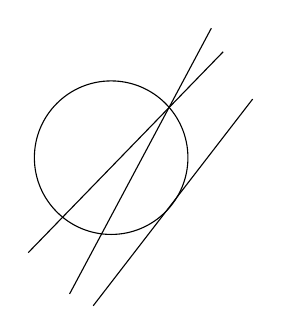
\begin{tikzpicture}[scale=0.3]
        % Coordinates
        \coordinate (A) at (4.51, 6.52);
        \coordinate (B) at (4.51, 6.52);
        \coordinate (C) at (1.00, 2.50);
        \coordinate (D) at (9.25, 11.00);
        \coordinate (E) at (2.75, 0.75);
        \coordinate (F) at (8.75, 12.00);
        \coordinate (G) at (3.75, 0.25);
        \coordinate (H) at (10.50, 9.00);

        % Drawing
        \draw (A) circle (3.25);
        \draw (C) -- (D);
        \draw (E) -- (F);
        \draw (G) -- (H);
    \end{tikzpicture}
    \caption{Secant lines through a circle (and a limiting tangent line)}\label{figure:secantexample}
\end{figure}
\begin{definition}[$r$-th Secant Variety to $X$]\label{defn:secantvariety}
    Let $X \subset \proj V$ be a projective variety. Then the $r$-th secant variety to $X$, denoted $\sigma_r(X)$ is defined as $$\sigma_r(X) := \overline{\bigcup_{x_1, \ldots, x_r \in X} \proj_{x_1, \ldots, x_r}}$$Here $\proj_{x_1, \ldots, x_r}$ (for $x_1, \ldots, x_r$ lying in general position) is the projectivisation of the $r$-dimensional hyperplane defined by these $r$ points. The bar denotes the Zariski closure in $\proj V$, covering the cases where the $r$ points chosen may not lie in general position, particularly also when all the $r$ chosen points coincide leading to the corresponding tangent hyperplane.
\end{definition}
\begin{observation}
    It is clear from the definition above that successive secant varieties are nested, with $\sigma_0(X) = X$, $\sigma_1(X)$ describing all the tangent lines to $X$, and so on, such that $\sigma_{r-1}(X) \subseteq \sigma_r(X)$. Such a sequence of nested geometric objects must stabilise, for reasons of dimension. 
\end{observation}
\begin{remark}
    While this geometric object is easy to describe with the notation above, computing the ideals for such a variety, or even the equations required to cut such a variety out form about half of the body of work surrounding Comon's conjecture. The following papers \cite{buczynska_secant_2013,buczynski_ranks_2013,bernardi_waring_2020} develop alternative geometric tools to secant varieties that are easier to compute.
\end{remark}
Since elementary tensors can be seen as lying on either the Segre or Veronese embedding, the $r$-th secant varieties to each of these describe all the tensors of \textit{border rank} at most $r$. Note here that it is border rank that because of the closure in the definition of the secant variety. To describe all tensors of \textit{rank} at most $r$, it is enough to look at the \textit{interior} points of the $r$-th secant variety, this interior again being under the Zariski topology on $\proj V$. 

% In fact \cite{bernardi_hitchhiker_2018} provides a comprehensive guide to the study of secant varieties, and highlights the importance of the Alexander-Hirschowitz theorem in computing the dimension of secant varieties. As previously observed, since secant varieties are nested, finding the first secant variety that covers all points in projective space allows for an upper bound on the length of all decompositions of tensors. This allows for the computation of "generic" rank

\section{Overview of Symmetric Tensor Decomposition}\label{section:pastoverview}
As mentioned in the introduction Comon et al. \cite{comon_symmetric_2008} showed symmetric rank and rank coincided for tensors of "large enough" order --- a notion that became concrete in later literature. The authors also point out as a result of the Veronese embedding (see \cref{defn:veronesemapping}), the rank of a symmetric tensor $T \in S^d(\complex^n)$ cannot be more than $\binom{n + d - 1}{d}$. 

% What is generic rank? -> Generic Rank in $S^d(\field^n)$ known for all values $d, n$ because of Alexander and Hirschowitz.

Since $S^d(\complex^n) \subseteq (\complex^{n})^{\otimes d}$, they pointed out that for all $T \in S^d(\complex^n)$, $\rank(T) \leq \srank(T)$. Their major result was that the conjecture holds "generically" (i.e almost everywhere) whenever $\srank(T) \leq n$, the dimension of the underlying vector space. In fact for every $T\in S^d(\complex^n)$, they showed that Comon's conjecture holds if $\srank(T) = 1,2$.

% Here the term generic (and typical) have specific mathematical meanings. Generic is used for a property that holds almost everywhere, whereas typical properties hold on non-zero volume sets. Such a distinction is not particularly pertinent over $\complex$, but may vary over other fields. 
Brachat et al. \cite{brachat_symmetric_2010}, in 2010 proposed a new algorithm for symmetric tensor decomposition beginning with the relationship between symmetric tensor decomposition and the secant varieties of a Veronese variety (see Section \cref{section:secantvarieties}). Their resulting algorithm required a reformulation of the problem in a dual space, and Hankel operators.[INCLUDE THIS?]

A convergent approach to Comon's conjecture arises from a classical problem in number theory --- the Waring decomposition of a number. This problem then gets restated into the Waring problem for polynomials as follows: \textit{What is the the minimum number of linear polynomials required such that a linear combination of them to the $d$th power is equal to a homogenous degree $d$ polynomial?} 

A solution to the polynomial Waring problem definitely solves the first issue of computing symmetric tensor decompositions (see \cref{subsection:homogenouspolyrelation}). This problem was solved by Alexander and Hirschowitz in 1995, where they showed that $\sigma_r(\nu_d(\proj \field^{n+1}))$ - the $r$-th secant variety to the $d$-th Veronese embedding of $\field^{n+1}$ - is of expected dimension with 5 exceptional cases. Brambilla and Ottaviani \cite{brambilla_alexanderhirschowitz_2008} in 2008 gave a self-contained proof of the theorem, with some simplifications, particularly in the case of order $3$ symmetric tensors.

Landsberg \cite{landsberg_tensors_2012}, in his textbook describes the conjecture in terms of (border) rank preserving pairs of projective varieties. 
\begin{definition}[(Border) Rank Preserving Pair]\label{defn:brpp}
    $X \subseteq \proj V$, a variety, and $L \subseteq \proj V$ a linear subspace when taken together as $(X,L)$ are a \textit{(border) rank preserving pair} if $\langle(X \cap L)_{red}\rangle = L$ and $\rank(X|_L) = \rank(X|_{(X \cap L)_{red}})$. (A similar condition holds for border rank, but this can now be stated in terms of secant varieties as $\sigma_r(X) \cap L = \sigma_r((X\cap L)_{red}))$. Here $(X\cap L)_{red}$ refers to the intersection without any points of non-unit multiplicity. and $\rank$ is now seen as a function from $\langle X \rangle \to \naturals$
\end{definition}
\begin{remark}
    This translates the statement of Comons conjecture from algebra to a statement about (secant) varieties lying in some projective space. In this restatement, $\Sigma(\proj \field^n \times \cdots \times \proj \field^n)$ (the $d$-fold Segre embedding) and $\proj(S^d(\field^n))$ (all the lines passing through the $d$-th Veronese) are required to be a rank-preserving pair.
\end{remark}
% One of the major issues with trying to work on Comon's conjecture via the world of geometry is the fact that computing the defining equations for secant varieties involves computin determinants or minors, which is computationally quite expensive/prohibitive.

Ballico and Bernardi \cite{ballico_tensor_2013} in 2013 showed that that tensors lying on the tangent variety to a Veronese variety (see \cref{defn:veronesemapping}) must always have $\rank = \srank$. Their proof highlighted explicit algorithms for the computation of the rank of a tensor belonging to a given secant variety. Their computation involves describing how a point on the tangent variety can be expressed by lying on the linear span of a degree 2 zero-dimensional scheme.


% In the literature reviewed, one of the most popular techniques used to compute the symmetric rank of a given order $d$ tensor is the construction of \textit{secant varieties} to the Veronese variety $\nu_d(\proj \field^n)$ --- since this variety describes all the elementary order-$d$ symmetric tensors geometrically. Points lying on the $r$-th secant variety to such a construction are guaranteed to have symmetric rank $r$ (Exceptions are covered by the Alexander-Hirschowitz theorem, that describes the discrepancy between expected rank and actual rank for symmetric tensors \cite{brambilla_alexanderhirschowitz_2008}.) 

While secant varieties are convenient geometric tools to use, Buczynska and Buczynski\cite{buczynska_secant_2013} demonstrate how the commonly used practice of using the $(r+1) \times (r+1)$ minors of the \textit{catalecticant matrix} to compute the generating equations for the secant variety are not sufficient for higher order Veronese varieties (order $>> 2$). This paper resulted in the developement of \textit{cactus varieties.}

Oeding and Ottaviani \cite{oeding_eigenvectors_2013} in 2013 contributed new algorithms for computing solutions to the polynomial Waring decomposition problem - equivalent to the computation of secant varieties to a given Veronese variety. They did so by further developing work done to define the eigenvectors of a tensor. Using these eigenvectors and Kozul flattenings allowed for an algorithm that could compute the Waring decomposition while also remaining valid for previously covered cases under the catalecticant matrix methodology.

Computing decompositions covers one half of the questions about symmetric rank. The other half concerning the uniqueness of a decomposition requires the definition of when a tensor is \textit{identifiable}. 

\begin{definition}[Identifiability]\label{defn:identifiability}
    A tensor $T$ is said to be identifiable if it admits only one rank decomposition (modulo scaling by $d$-th roots of unity and permutations of summands)
\end{definition}
\begin{observation}
    This definition is equivalent to asking that an identifiable tensor lie on only one secant variety (again modulo permutations of points on the Segre embedding, and scaling factors)
\end{observation}
Identifiability is a useful property when working with symmetric tensors because no further computation is required once a tensor decomposition is found. Particularly for the case of Comon's conjecture, the distinction between rank and symmetric rank (if such a tensor exists) implies that the tensor in question is \textit{not} identifiable. 

Generic identifiability is the idea that almost every point (i.e. a point in a dense open subset), is identifiable. Specific identifiability poses the opposite question - given a specific tensor $T$, does it admit a unique decomposition? Chiantini, Ottaviani and Vannieuwenhoven \cite{chiantini_generic_2016, chiantini_effective_2017} in 2 subsequent papers tackled both of these questions. Their earlier paper showed that a general symmetric tensor in $S^d(\complex^{n+1})$ of sub-generic rank $r$ was identifiable, provided $r \leq \binom{n+d}{d}/(n+1)$ (with exceptions again being covered by the Alexander-Hirschowitz theorem). Their second paper focused on showing what criteria could be called "effective" to determine if a given tensor was specifically identifiable. Criteria were designated effective if their conditions were satisfied by generic points (i.e. they were satisfied in an open, dense subset). One of the conclusions this paper reacheed was that Kruskal's criterion fell in line with this definition of "effectiveness". 

Friedland \cite{friedland_remarks_2016} in 2016 focused not on the computation of the symmetric rank, but on the properties of symmetric tensors of a given symmetric rank. In particular the paper focuseed on showing that when a symmetric tensor can be unfolded into a matrix (see \cref{subsection:tensorflattening}), then Comon's Conjecture held if the rank of the tensor when computed was either the rank of the matrix or the rank of the matrix $+1$. 

Zhang et al. \cite{zhang_comons_2016} conclusively showed that Comon's conjecture held for all tensors where the rank of the tensor under consideration is not more than its order.

% Carlini et al. \cite{carlini_real_2017} in 2017 discussed the computation of real and complex rank for symmetric tensors associated to monomials of a fixed degree, and showed that these must agree when the least exponent in the monomial is 1. They did so by using duals to the homogenous ring of polynomials to describe a differentiation operation, giving rise to ideals that were "perpendicular" to any one monomial under scrutiny.

Ballico et al \cite{ballico_bounds_2018} at the end of 2018, refocused on the question of identifiability, and worked on refining Kruskals criterion (sharp and algebraic in nature) into a geometric criterion that can be verified more easily. They concluded that Comon's conjecture holds for general tensors whose symmetric rank $r$ is bounded above strictly by $\binom{n+e}{e}$ for a specific choice of $e$. This choice depended upon splitting the Segre product into two disjoint components and then imposing conditions on a set of points on the Segre that exhibited distinct behavious when projected down to the first component versus the second . The authors of this paper clearly point out that even though they have increased the scope of validity of Comon's conjecture, Shitov's proposed counterexample \cite{shitov_counterexample_2018} lies outside this scope and thus might have still been a plausible counterexample.

Bernardi et al. \cite{bernardi_hitchhiker_2018} in 2018 comprehensively covered the literature and algorithms required to understand how secant varieties become useful in establishing questions about (generic) rank for tensors, with an emphasis on symmetric tensors and the mapping to the Veronese variety.

Casarotti et al. \cite{casarotti_comons_2018} proposed to improve the bounds for Comon's conjecture when working with flattenings, provided that equations for the secant varieties associated to the Veronese variety could be generated. Their result was that $h < \binom{n + \lfloor \frac{d}{2} \rfloor}{n}$, for a tensor having rank $h$ implies that $\srank = h$, for cases where such generating determinantal equations were known.

Finally in \cite{seigal_ranks_2020} Seigal demonstrated that for all "cubic surfaces", Comon's conjecture does hold. (even up to border rank.) Here cubic surfaces were used to refer to the fact that under the identification with homogenous polynomials, order $3$ symmetric tensors correspond to cubic polynomials, and thus their zero sets could be called cubic surfaces. She also used flattenings of tensors (see \cref{subsection:tensorflattening}), dividing her proof into cases depending on the number of singularities on the cubic surfaces in question.

% Strassen's conjecture: Determining the algorithmic complexity of matrix multiplication. Does there exist a tensor decomposition that computes two distinct matrix multiplications that costs less (has less rank) than the sum of the matrix multiplications individually? Additivity holds for bilinear maps \cite{landsberg_tensors_2012}
\section{Overview of Valid Cases of the Conjecture}\label{section:validoverview}
The current overview of the cases where Comon's Conjecture holds so far is as follows: \begin{itemize}
	\item For $T = \sum_{i=1}^{s} y_i^{\otimes d}$ and $d$ "large enough" \cite{comon_symmetric_2008}. Here the large enough argument in the paper hinges on a classical result from algebraic geometry, stating that $d$ points in $\complex^n$ form the solution set of of polynomial equations of degree $\leq d$
	\item For $T \in S^d(\complex^n)$ and $\text{rank}_S(T) = 1, 2$ \cite{comon_symmetric_2008}
	\item For $T \in S^d{V}$, and rank$(T) \leq \frac{dn - d + 1}{2}$ where $V$ is a real or complex vector space with dimension $n$ \cite{oeding_report_2008}
	\item For $T \in S^d(\complex^n)$ for $(d,n) \in \{(3,2), (4,2), (3,3)\}$ \cite{friedland_remarks_2016}
	\item In the case $d \geq 3, | \mathbb{F} | \geq 3, T \in S^d(\mathbb{F}^n)$ and rank$(T) \leq$ rank$U(T) + 1$ (Here $U$ denotes the flattening \cref{subsection:tensorflattening}  of $T$ in any direction, since $T$ is symmetric all directions are equivalent) \cite{friedland_remarks_2016}
	\item When $T \in S^3(\complex^n)$ and rank$(T) \leq 5$ or rank$_S(T) \leq 6$ \cite{friedland_remarks_2016}
	\item For $T \in S^d(\mathbb{F}^n)$ where rank$(T) \leq d$ where $\mathbb{F} = \reals , \complex$\cite{zhang_comons_2016}
	\item If $T$ is a tensor belonging to a tangential variety to a Veronese variety \cite{ballico_tensor_2013}
	\item If $T \in \complex^2 \otimes \complex^n \otimes \complex^n$ \cite{buczynski_ranks_2013}
	\item For $T$ being a Coppersmith-Winograd tensor \cite{landsberg_abelian_2017}
	\item Casarotti \cite{casarotti_comons_2018} sets up two propositions that suggest whenever determinantlal equations for secant varieties can be written down, Comon's conjecture should be \textit{verifiable}
	\item Whenever a tensor $T$ is cubic surface (real or complex) \cite{seigal_ranks_2020}
\end{itemize}

\chapter{Constructions required for a Counterexample}\label{chapter:constructionsrequired}
\section{History}\label{section:historyconstructions}
In spite of all of these preliminary results that indicate positive answers towards Comon's Conjecture, Yaroslav Shitov seemed to arrive at a method of constructing a counterexample, as early as 2019 \cite{shitov_counterexample_2018}. An apparent error found in this paper leads to an inalidation of this result in 2024, but the period of 5 years in the interim led to multople other preprints from Shitov, starting with a newer, alternate methodology for the construction of counterexamples. Therefore, while there is now no material carrying the stamp of peer-review and Shitov's name, his contributions and subsequent papers seem to indicate a viable approach to disproving Comon's conjecture, at least over $\reals$ if not $\complex$.   
\subsection{Shitov's First Paper in 2019}\label{section:shitovpaper}
The 2018 paper begins with taking the ground field as $\complex$, and fixing the notation to be used. The main objects of interest are order $3$ tensors, and the introductory section of the paper highlights the behavious of such tensors under elementary transformations with respect to their constituent order $2$ "slices" (see \cref{subsection:tensorslicing}). The construction of the counterexample begins in earnest with the description of a $100 \times 100$ matrix, partitioned into 20 submatrices. Each submatrix then is mapped to a corresponding $100 \times 100$ matrix, now with entries in the submatrix seen as $1$ and all other entries as $0$. Now taking the $1-$ and $2-$ supports of each of these, and pre and post multiplying them with the column shift operator with parameter $a$ Leads to another set of matrices of similar size (still $100 \times 100$).

It is at this point that the paper makes a construction that seems strange. A set is constructed consisting of matrices of distinct orders (viz. $200 \times 200$ and $400 \times 400$). While there is no issue in defining such a set, the paper then asks for the construction of "the $\complex$-linear span" of the elements of this set. Addition of quantities that do not live in the same dimension (at least from this author's prior knowledge), without a specified or implied embedding map presents the first major problem when following this construction.

These instructions illustrate the procedure to be followed, but further in the paper a tensor decomposition is claimed to exist of the following form
 $$\mathcal{S} - \Phi = \Xi_1 + \Xi_2 + \Xi_3 + \sum_{b \in \mathcal{B}'} (\Xi_b^1 + \Xi_b^2 + \Xi_b^3)$$. This statement (no context is necessary for the symbols used, they indicate tensors of appropriate formats being combined) is the subject of the erratum published in 2024 \cite{draisma_erratum_2024} indicating such a statement was true only for trivial cases of all the terms on the RHS being $0$, but equality could not be said to hold in general otherwise without proof. This crucial observation led to the invalidation of this entire construction.

 While certain choices were made during this process that led to unanswered questions, the overall tools for establishing a counterexample were first established in this paper. These include the two minor operations - slicing tensors (\cref{subsection:tensorslicing}) and flattening tensors (\cref{subsection:tensorflattening}) and the three major operations - adjoining slices to tensors (\cref{subsection:adjoiningslices}), generating families modulo slices (\cref{subsection:familymoduloslices}) and cloning (\cref{subsection:tensorcloning}).  
\subsection{Shitov's Subsequent Preprints}\label{section:shitovpreprints}

In the following years, Shitov put out a number of preprints \cite{shitov_comons_2020,shitov_higher_2024,shitov_higher_2024-1} each either tackling Comon's conjecture in a restricted setting, or developing tools to construct more general counterexamples, that might also be used to construct a counterexample to Strassen's conjecture (another rank conjecture concerning the additivity of rank.) The preprint from 2020 \cite{shitov_comons_2020} tackles the conjecture over $\reals$ and it is this that forms the basis for the paper \cite{wang_lower_2023}.

The constructions made in each preprint follow the same pattern, indicating a common toolset and structure of approach. Each approach sees an order $d$ tensor as composed of lower order $d-1$ tensors, which allows for tensors to be transformed per slice along a particular direction. Viewing tensors in this way opens up a way to describe tensors modulo these slices --- useful and seen in both number theory and algebraic geometry as a tool to study problems in a more restricted setting. Such a family, when generated, gives an idea of the general properties of the orginal tensor (how many linearly independent slices in which direction etc.) Flatness as a tool comes in to help with the computation of rank for these slices (since computing the rank of matrices is a known and easier problem to solve than for higher order matrices), and lends itself to descrbing rank information that changes in the relationship between a tensor and its slices.

These tools allow for an analysis of any particular tensor, but the "construction" aspect of this approach becomes evident with the adjoining of slices to a tensor. This operation changes the format of the original tensor with respect to certain "important" slices, and allows for the rank information of the family generated modulo the slices to be preserved in a new tensor that now contains both the original and the slices that are required.

Cloning starts to play a role when such an adjoined tensor even if it has the properties required, but any perturbation of such a constructed tensor (usually by the modification of one of the constituent slices) causes a violation of the properties that were supposed to be preserved. Cloning is a way to maintain rank information by simply making a higher format copy, and allows for more "freedom".

While each of these preprints starts with this general structure, and \cite{shitov_higher_2024-1} in particular proposes the construction of a general counterexample over any $\field$ with $\text{char}(\field) \neq 2,3$, an intermediate step involved in all of these is the construction of an "emulating family". Such a family, if it exists, allows for the rest of the constructions to proceed. However, proving the existence of such a family is not trivial. The latest preprint does attempt to do so, highlighting a similar construction from \cite{shitov_higher_2024}, but tracing the construction back leads to the definition of a function dependent on an arbitrary constant - much in the same way as the paper \cite{shitov_counterexample_2018} relied on the existence of an arbitrarily partitioned $100 \times 100$ matrix. Such choices, while they may be valid, did not appear to be explained at any point in their corresponding documents, raising some skepticism and prompting further investigation into alternate methods that could explain their existence, or proofs that could deny their existence.
\subsection{Slicing a Tensor}\label{subsection:tensorslicing}
The viewing of the columns or rows of a matrix as linearly dependent or independent and how they affect the overall linear transformation described by the matrix is the exact low-order analogue for describing tensors as composed of slices. Conventionally the columns of a matrix would be the $1$ slices.
\begin{definition}[Slices of a Tensor]\label{defn:tensorslicing}
    Let $T \in \mathbb{F}^{n_1} \otimes \cdots \otimes \mathbb{F}^{n_d}$ be an order $d$ tensor. Then the $j$-th $i$ slices of $T$ are given by $$T_j^i:= f_j(v_i)(v_1 \otimes \cdots v_{i-1} \otimes v_{i+1} \cdots \otimes v_d)$$ $f_j(v_i)$ denotes the $j$th component of $v_i$ and $1 \leq j \leq n_i$. For each \textit{mode} $1 \leq i \leq d$, there are $n_i$ order $d-1$ \textit{slices} that make up $T$. 
\end{definition}
\begin{figure}[h]
    \centering
    \begin{tikzpicture}[scale=0.9]
        \definecolor{darkgreen}{RGB}{0,113,0}

        % Coordinates
        \coordinate (A) at (1.00, 8.00);
        \coordinate (B) at (1.97, 9.00);
        \coordinate (C) at (4.00, 8.00);
        \coordinate (D) at (4.98, 9.02);
        \coordinate (E) at (4.00, 4.00);
        \coordinate (F) at (5.00, 5.00);
        \coordinate (G) at (1.50, 8.50);
        \coordinate (H) at (4.50, 8.50);
        \coordinate (I) at (4.50, 4.50);
        \coordinate (J) at (2.00, 8.00);
        \coordinate (K) at (2.00, 4.00);
        \coordinate (L) at (3.00, 8.00);
        \coordinate (M) at (3.00, 4.00);
        \coordinate (N) at (3.00, 9.00);
        \coordinate (O) at (4.00, 9.00);
        \coordinate (P) at (1.00, 7.00);
        \coordinate (Q) at (4.00, 7.00);
        \coordinate (R) at (5.00, 8.00);
        \coordinate (S) at (1.00, 6.00);
        \coordinate (T) at (4.00, 6.00);
        \coordinate (U) at (5.00, 7.00);
        \coordinate (V) at (1.00, 5.00);
        \coordinate (W) at (4.00, 5.00);
        \coordinate (X) at (5.00, 6.00);
        \coordinate (Y) at (1.71, 9.51);
        \coordinate (Z) at (6.00, 7.00);
        \coordinate (AA) at (9.00, 10.00);
        \coordinate (AB) at (7.25, 7.00);
        \coordinate (AC) at (7.75, 10.00);
        \coordinate (AD) at (12.97, 7.04);
        \coordinate (AE) at (7.50, 7.00);
        \coordinate (AF) at (7.50, 7.00);
        \coordinate (AG) at (9.00, 4.00);
        \coordinate (AH) at (8.25, 7.00);
        \coordinate (AI) at (7.25, 4.00);
        \coordinate (AJ) at (10.53, 11.97);
        \coordinate (AK) at (15.04, 9.10);
        \coordinate (AL) at (14.13, 3.55);

        % Drawing
        \draw (1,4) rectangle (4,8);
        \draw (A) -- (B);
        \draw (C) -- (D);
        \draw (E) -- (F);
        \draw[darkgreen] (B) -- (D);
        \draw[darkgreen] (F) -- (D);
        \draw[darkgreen, dashed] (G) -- (H);
        \draw[darkgreen, dashed] (H) -- (I);
        \draw[blue, dashed] (J) -- (K);
        \draw[blue, dashed] (L) -- (M);
        \draw[blue, dashed] (J) -- (N);
        \draw[blue, dashed] (L) -- (O);
        \draw[dashed] (P) -- (Q);
        \draw[dashed] (Q) -- (R);
        \draw[red, dashed] (S) -- (T);
        \draw[red, dashed] (T) -- (U);
        \draw[red, dashed] (V) -- (W);
        \draw[red, dashed] (W) -- (X);
        \node[above] at (Y) {$T \in \mathbb{F}^4 \otimes \mathbb{F}^3 \otimes \mathbb{F}^2$};
        \draw (Z) .. controls (7.25, 7.00) and (7.75, 10.00) .. (AA);
        \draw (Z) .. controls (7.50, 7.00) and (7.50, 7.00) .. (AD);
        \draw[red] (9.5,9) rectangle (11.5,12);
        \draw (13,9) rectangle (13,9);
        \draw[blue] (14,5) rectangle (16,9);
        \draw[darkgreen] (9.5,2) rectangle (12.5,6);
        \draw (Z) .. controls (8.25, 7.00) and (7.25, 4.00) .. (AG);
        \node[above] at (AJ) {$T^1_3 \in \mathbb{F}^3 \otimes \mathbb{F}^2$};
        \node[above] at (AK) {$T^2_2 \in \mathbb{F}^4\otimes \mathbb{F}^2$};
        \node[above] at (AL) {$T^3_2 \in \mathbb{F}^4\otimes \mathbb{F}^3$};
    \end{tikzpicture}
    \caption{Slicing a tensor $T$ along different modes}\label{figure:slicingtensor}
\end{figure}
\begin{observation}
    Through the rest of this thesis, the superscript accompanying a tensor variable indicates the mode chosen along which any operation must occur. \Cref{figure:slicingtensor} indicates how a tensor can be sliced along different modes, and how slicing along each mode results in lower order tensors of appropriate format.
\end{observation}
\begin{observation}
    Slicing in the above definition is described for only an elementary order $d$ tensor, but it is a linear operation (addition and scalar multiplication don't change it.)
\end{observation}
\begin{lemma}
    Given a tensor $T$ such that $\rank(T) = r$, then there is at least one mode $1 \leq i \leq d$ having $r$ linearly independent slices $T^i_j$ where $1 \leq j \leq n_i$.
\end{lemma}
What other major theorems/lemmas do we need to establish about slicing tensors?
What are the properties of slicing?
What does slicing look like in geometry?
\subsection{Flattening a Tensor}\label{subsection:tensorflattening}
Flattening, while not as important in Shitov's constructions, is an important operation to verify rank information for tensors. Such an operation can generally be used as a sanity check when performing operations or constructions on tensors.
\begin{definition}[Flattening a Tensor]\label{defn:tensorflattening}
    Let $T \in V_1 \otimes \cdots \otimes V_d$,  be an order $d$ tensor, such that $T = v_1 \otimes \cdots \otimes v_d$. Define $T^{(i)}$, the $i$-th flattening as follows $$T^{(i)}((k_1, \ldots k_{i-1},k_{i+1} \ldots k_d)|k_i) := T(k_1| k_2 | \ldots | k_d)$$
\end{definition}
\begin{figure}[h]
    \centering
    \begin{tikzpicture}[scale=1]
        % Coordinates
        \coordinate (A) at (1.00, 8.00);
        \coordinate (B) at (1.97, 9.00);
        \coordinate (C) at (4.00, 8.00);
        \coordinate (D) at (4.98, 9.02);
        \coordinate (E) at (4.00, 4.00);
        \coordinate (F) at (5.00, 5.00);
        \coordinate (G) at (1.50, 8.50);
        \coordinate (H) at (4.50, 8.50);
        \coordinate (I) at (4.50, 4.50);
        \coordinate (J) at (2.00, 8.00);
        \coordinate (K) at (2.00, 4.00);
        \coordinate (L) at (3.00, 8.00);
        \coordinate (M) at (3.00, 4.00);
        \coordinate (N) at (3.00, 9.00);
        \coordinate (O) at (4.00, 9.00);
        \coordinate (P) at (1.00, 7.00);
        \coordinate (Q) at (4.00, 7.00);
        \coordinate (R) at (5.00, 8.00);
        \coordinate (S) at (1.00, 6.00);
        \coordinate (T) at (4.00, 6.00);
        \coordinate (U) at (5.00, 7.00);
        \coordinate (V) at (1.00, 5.00);
        \coordinate (W) at (4.00, 5.00);
        \coordinate (X) at (5.00, 6.00);
        \coordinate (Y) at (1.49, 9.29);
        \coordinate (Z) at (6.25, 7.00);
        \coordinate (AA) at (8.25, 7.00);
        \coordinate (AB) at (6.92, 7.80);
        \coordinate (AC) at (7.50, 6.25);
        \coordinate (AD) at (10.47, 11.28);
        \coordinate (AE) at (11.47, 11.28);
        \coordinate (AF) at (12.47, 11.28);
        \coordinate (AG) at (9.50, 10.25);
        \coordinate (AH) at (9.50, 9.25);
        \coordinate (AI) at (9.50, 8.25);
        \coordinate (AJ) at (9.50, 3.25);
        \coordinate (AK) at (9.50, 6.00);
        \coordinate (AL) at (11.50, 2.25);
        \coordinate (AM) at (11.00, 11.00);
        \coordinate (AN) at (11.00, 3.00);
        \coordinate (AO) at (12.00, 11.00);
        \coordinate (AP) at (12.00, 3.00);
        \coordinate (AQ) at (9.99, 10.02);
        \coordinate (AR) at (12.99, 10.02);
        \coordinate (AS) at (10.00, 9.00);
        \coordinate (AT) at (13.00, 9.00);
        \coordinate (AU) at (10.00, 8.00);
        \coordinate (AV) at (13.00, 8.00);
        \coordinate (AW) at (10.00, 7.00);
        \coordinate (AX) at (13.00, 7.00);
        \coordinate (AY) at (10.00, 6.00);
        \coordinate (AZ) at (13.00, 6.00);
        \coordinate (BA) at (10.00, 5.00);
        \coordinate (BB) at (13.00, 5.00);
        \coordinate (BC) at (10.00, 4.00);
        \coordinate (BD) at (13.00, 4.00);

        % Drawing
        \draw (1,4) rectangle (4,8);
        \draw (A) -- (B);
        \draw (C) -- (D);
        \draw (E) -- (F);
        \draw (B) -- (D);
        \draw (F) -- (D);
        \draw[dashed] (G) -- (H);
        \draw[dashed] (H) -- (I);
        \draw[dashed] (J) -- (K);
        \draw[dashed] (L) -- (M);
        \draw[dashed] (J) -- (N);
        \draw[dashed] (L) -- (O);
        \draw[dashed] (P) -- (Q);
        \draw[dashed] (Q) -- (R);
        \draw[dashed] (S) -- (T);
        \draw[dashed] (T) -- (U);
        \draw[dashed] (V) -- (W);
        \draw[dashed] (W) -- (X);
        \node[above] at (Y) {$T \in \mathbb{F}^4 \otimes \mathbb{F}^3 \otimes \mathbb{F}^2$};
        \draw (Z) .. controls (6.92, 7.80) and (7.50, 6.25) .. (AA);
        \draw (10,3) rectangle (13,11);
        \node[above] at (AD) {$1$};
        \node[above] at (AE) {$2$};
        \node[above] at (AF) {$3$};
        \node[above] at (AG) {$1,1$};
        \node[above] at (AH) {$1,2$};
        \node[above] at (AI) {$2,1$};
        \node[above] at (AJ) {$4,2$};
        \node[above] at (AK) {$\vdots$};
        \node[above] at (AL) {$T^{(2)}$};
        \draw[dashed] (AM) -- (AN);
        \draw[dashed] (AO) -- (AP);
        \draw[dashed] (AQ) -- (AR);
        \draw[dashed] (AS) -- (AT);
        \draw[dashed] (AU) -- (AV);
        \draw[dashed] (AW) -- (AX);
        \draw[dashed] (AY) -- (AZ);
        \draw[dashed] (BA) -- (BB);
        \draw[dashed] (BC) -- (BD);
    \end{tikzpicture}
    \caption{Flattening a tensor  $T$}\label{figure:flatteningtensor}
\end{figure}
\begin{observation}
    Flattening $T$ to $T^{(i)}$ is the operation by which in \cref{section:tensoralgebra} $T$ could be seen as a linear map between vector spaces instead. Here $T^{(i)} \in V_{\hat{i}} \otimes V_i $, seen as a matrix, representing the mapping $V_i^* \to V_{\hat{i}}$ Each column $T^{(i)}_j := T^{(i)}(\ldots | j)$ represents the flattening of the $j$-th $i$ slice of $T$, or $(T_j^i)^{\emptyset}$. \Cref{figure:flatteningtensor} illustrates how a tensor of higher order can be flattened, and also indicates how the row and column indices are derived for the new matrix. 
\end{observation}
What kind of operation is flattening?
Graphically what does flattening describe?
\section{Major New Constructions}\label{section:majorconstructions}
\subsection{Adjoining Slices to Tensors}\label{subsection:adjoiningslices}
\begin{figure}
    \centering
    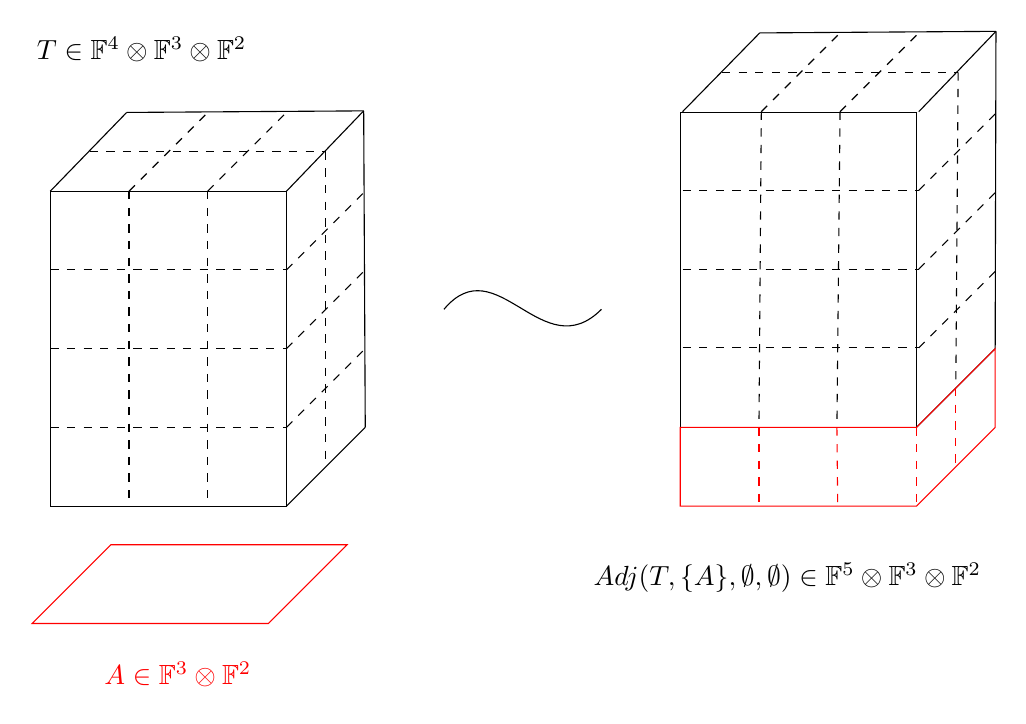
\begin{tikzpicture}[scale=1]
        % Coordinates
        \coordinate (A) at (1.00, 8.00);
        \coordinate (B) at (1.97, 9.00);
        \coordinate (C) at (4.00, 8.00);
        \coordinate (D) at (4.98, 9.02);
        \coordinate (E) at (4.00, 4.00);
        \coordinate (F) at (5.00, 5.00);
        \coordinate (G) at (1.50, 8.50);
        \coordinate (H) at (4.50, 8.50);
        \coordinate (I) at (4.50, 4.50);
        \coordinate (J) at (2.00, 8.00);
        \coordinate (K) at (2.00, 4.00);
        \coordinate (L) at (3.00, 8.00);
        \coordinate (M) at (3.00, 4.00);
        \coordinate (N) at (3.00, 9.00);
        \coordinate (O) at (4.00, 9.00);
        \coordinate (P) at (1.00, 7.00);
        \coordinate (Q) at (4.00, 7.00);
        \coordinate (R) at (5.00, 8.00);
        \coordinate (S) at (1.00, 6.00);
        \coordinate (T) at (4.00, 6.00);
        \coordinate (U) at (5.00, 7.00);
        \coordinate (V) at (1.00, 5.00);
        \coordinate (W) at (4.00, 5.00);
        \coordinate (X) at (5.00, 6.00);
        \coordinate (Y) at (2.16, 9.52);
        \coordinate (Z) at (9.03, 9.01);
        \coordinate (AA) at (10.01, 10.01);
        \coordinate (AB) at (12.03, 9.01);
        \coordinate (AC) at (13.01, 10.03);
        \coordinate (AD) at (12.00, 5.00);
        \coordinate (AE) at (13.00, 6.00);
        \coordinate (AF) at (9.53, 9.51);
        \coordinate (AG) at (12.53, 9.51);
        \coordinate (AH) at (12.50, 5.50);
        \coordinate (AI) at (10.03, 9.01);
        \coordinate (AJ) at (10.00, 5.00);
        \coordinate (AK) at (11.03, 9.01);
        \coordinate (AL) at (10.99, 5.00);
        \coordinate (AM) at (11.03, 10.01);
        \coordinate (AN) at (12.03, 10.01);
        \coordinate (AO) at (9.03, 8.01);
        \coordinate (AP) at (12.03, 8.01);
        \coordinate (AQ) at (13.03, 9.01);
        \coordinate (AR) at (9.03, 7.01);
        \coordinate (AS) at (12.03, 7.01);
        \coordinate (AT) at (13.03, 8.01);
        \coordinate (AU) at (9.03, 6.01);
        \coordinate (AV) at (12.03, 6.01);
        \coordinate (AW) at (13.03, 7.01);
        \coordinate (AX) at (0.77, 2.51);
        \coordinate (AY) at (3.77, 2.51);
        \coordinate (AZ) at (4.77, 3.51);
        \coordinate (BA) at (1.77, 3.51);
        \coordinate (BB) at (2.62, 1.58);
        \coordinate (BC) at (9.00, 5.00);
        \coordinate (BD) at (9.00, 4.00);
        \coordinate (BE) at (12.00, 4.00);
        \coordinate (BF) at (13.00, 5.00);
        \coordinate (BG) at (10.00, 4.00);
        \coordinate (BH) at (11.00, 4.00);
        \coordinate (BI) at (12.50, 4.50);
        \coordinate (BJ) at (10.36, 2.78);
        \coordinate (BK) at (6.00, 6.50);
        \coordinate (BL) at (8.00, 6.50);
        \coordinate (BM) at (6.67, 7.30);
        \coordinate (BN) at (7.25, 5.75);

        % Drawing
        \draw (1,4) rectangle (4,8);
        \draw (A) -- (B);
        \draw (C) -- (D);
        \draw (E) -- (F);
        \draw (B) -- (D);
        \draw (F) -- (D);
        \draw[dashed] (G) -- (H);
        \draw[dashed] (H) -- (I);
        \draw[dashed] (J) -- (K);
        \draw[dashed] (L) -- (M);
        \draw[dashed] (J) -- (N);
        \draw[dashed] (L) -- (O);
        \draw[dashed] (P) -- (Q);
        \draw[dashed] (Q) -- (R);
        \draw[dashed] (S) -- (T);
        \draw[dashed] (T) -- (U);
        \draw[dashed] (V) -- (W);
        \draw[dashed] (W) -- (X);
        \node[above] at (Y) {$T \in \mathbb{F}^4 \otimes \mathbb{F}^3 \otimes \mathbb{F}^2$};
        \draw (9,5) rectangle (12,9);
        \draw (Z) -- (AA);
        \draw (AB) -- (AC);
        \draw (AD) -- (AE);
        \draw (AA) -- (AC);
        \draw (AE) -- (AC);
        \draw[dashed] (AF) -- (AG);
        \draw[dashed] (AG) -- (AH);
        \draw[dashed] (AI) -- (AJ);
        \draw[dashed] (AK) -- (AL);
        \draw[dashed] (AI) -- (AM);
        \draw[dashed] (AK) -- (AN);
        \draw[dashed] (AO) -- (AP);
        \draw[dashed] (AP) -- (AQ);
        \draw[dashed] (AR) -- (AS);
        \draw[dashed] (AS) -- (AT);
        \draw[dashed] (AU) -- (AV);
        \draw[dashed] (AV) -- (AW);
        \draw[red] (AX) -- (AY) -- (AZ) -- (BA) -- cycle;
        \node[above, text=red] at (BB) {$A \in \mathbb{F}^3 \otimes \mathbb{F}^2
        $};
        \draw[red] (BC) -- (BD) -- (BE) -- (BF) -- (AE) -- (AD) -- cycle;
        \draw[red, dashed] (AJ) -- (BG);
        \draw[red, dashed] (AL) -- (BH);
        \draw[red, dashed] (AD) -- (BE);
        \draw[red, dashed] (AH) -- (BI);
        \node[above] at (BJ) {$Adj(T, \{A\}, \emptyset, \emptyset)\in \mathbb{F}^5\otimes\mathbb{F}^3\otimes\mathbb{F}^2$};
        \draw (BK) .. controls (6.67, 7.30) and (7.25, 5.75) .. (BL);
    \end{tikzpicture}
    \caption{Adjoining a slice $A$ to a tensor $T$}\label{figure:adjoiningslices}
\end{figure}
\subsection{Generating Tensor Families modulo Slices}\label{subsection:familymoduloslices}
\begin{figure}
    \centering
    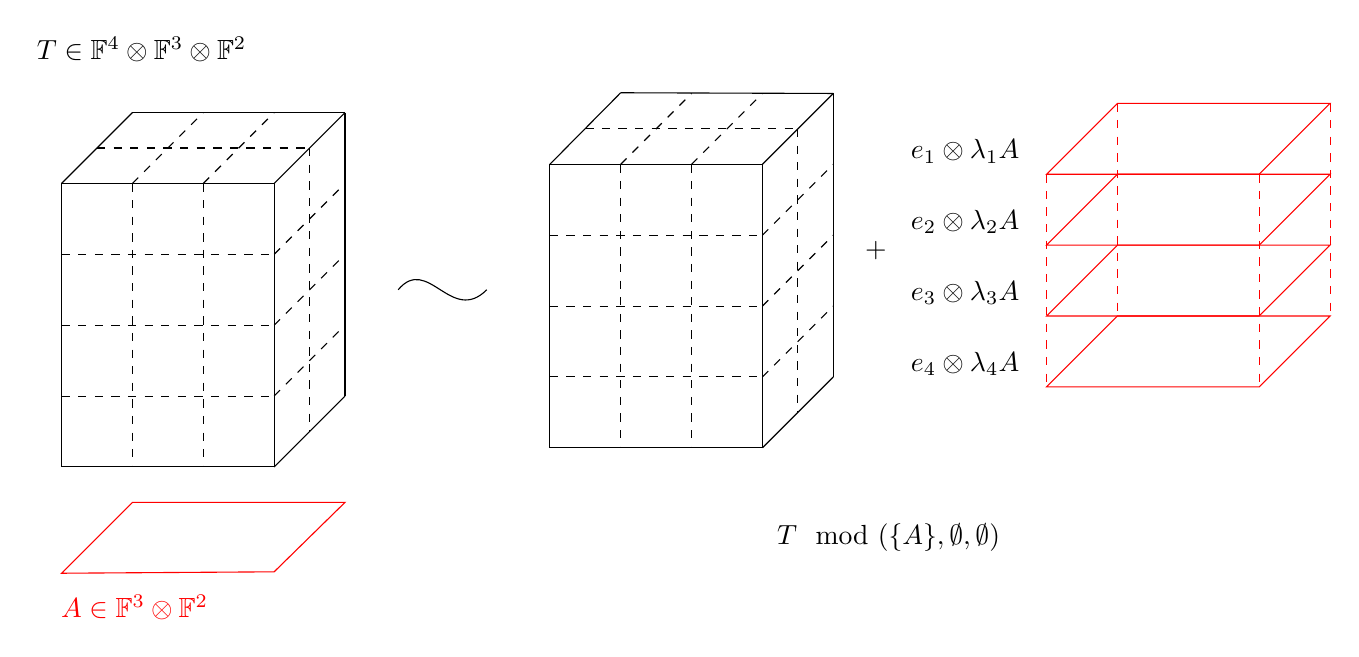
\begin{tikzpicture}[scale=0.9]
        % Coordinates
        \coordinate (A) at (1.00, 8.00);
        \coordinate (B) at (2.00, 9.00);
        \coordinate (C) at (4.00, 8.00);
        \coordinate (D) at (5.00, 9.00);
        \coordinate (E) at (4.00, 4.00);
        \coordinate (F) at (5.00, 5.00);
        \coordinate (G) at (1.50, 8.50);
        \coordinate (H) at (4.50, 8.50);
        \coordinate (I) at (4.50, 4.50);
        \coordinate (J) at (2.00, 8.00);
        \coordinate (K) at (2.00, 4.00);
        \coordinate (L) at (3.00, 8.00);
        \coordinate (M) at (3.00, 4.00);
        \coordinate (N) at (3.00, 9.00);
        \coordinate (O) at (4.00, 9.00);
        \coordinate (P) at (1.00, 7.00);
        \coordinate (Q) at (4.00, 7.00);
        \coordinate (R) at (5.00, 8.00);
        \coordinate (S) at (1.00, 6.00);
        \coordinate (T) at (4.00, 6.00);
        \coordinate (U) at (5.00, 7.00);
        \coordinate (V) at (1.00, 5.00);
        \coordinate (W) at (4.00, 5.00);
        \coordinate (X) at (5.00, 6.00);
        \coordinate (Y) at (2.13, 9.58);
        \coordinate (Z) at (1.00, 2.50);
        \coordinate (AA) at (4.00, 2.52);
        \coordinate (AB) at (5.00, 3.50);
        \coordinate (AC) at (2.00, 3.50);
        \coordinate (AD) at (2.03, 1.71);
        \coordinate (AE) at (7.89, 8.27);
        \coordinate (AF) at (8.89, 9.28);
        \coordinate (AG) at (10.89, 8.27);
        \coordinate (AH) at (11.89, 9.27);
        \coordinate (AI) at (10.89, 4.27);
        \coordinate (AJ) at (11.89, 5.27);
        \coordinate (AK) at (8.39, 8.77);
        \coordinate (AL) at (11.39, 8.77);
        \coordinate (AM) at (11.39, 4.77);
        \coordinate (AN) at (8.89, 8.27);
        \coordinate (AO) at (8.89, 4.27);
        \coordinate (AP) at (9.89, 8.27);
        \coordinate (AQ) at (9.89, 4.27);
        \coordinate (AR) at (9.89, 9.27);
        \coordinate (AS) at (10.89, 9.27);
        \coordinate (AT) at (7.89, 7.27);
        \coordinate (AU) at (10.89, 7.27);
        \coordinate (AV) at (11.89, 8.27);
        \coordinate (AW) at (7.89, 6.27);
        \coordinate (AX) at (10.89, 6.27);
        \coordinate (AY) at (11.89, 7.27);
        \coordinate (AZ) at (7.89, 5.27);
        \coordinate (BA) at (10.89, 5.27);
        \coordinate (BB) at (11.89, 6.27);
        \coordinate (BC) at (14.90, 8.13);
        \coordinate (BD) at (17.90, 8.13);
        \coordinate (BE) at (18.90, 9.13);
        \coordinate (BF) at (15.90, 9.13);
        \coordinate (BG) at (14.90, 7.13);
        \coordinate (BH) at (17.90, 7.13);
        \coordinate (BI) at (18.90, 8.13);
        \coordinate (BJ) at (15.90, 8.13);
        \coordinate (BK) at (14.90, 6.13);
        \coordinate (BL) at (17.90, 6.13);
        \coordinate (BM) at (18.90, 7.13);
        \coordinate (BN) at (15.90, 7.13);
        \coordinate (BO) at (14.90, 5.13);
        \coordinate (BP) at (17.90, 5.13);
        \coordinate (BQ) at (18.90, 6.13);
        \coordinate (BR) at (15.90, 6.13);
        \coordinate (BS) at (5.75, 6.50);
        \coordinate (BT) at (7.00, 6.50);
        \coordinate (BU) at (6.17, 7.00);
        \coordinate (BV) at (6.50, 6.00);
        \coordinate (BW) at (12.49, 6.78);
        \coordinate (BX) at (13.75, 8.15);
        \coordinate (BY) at (13.75, 7.15);
        \coordinate (BZ) at (13.75, 6.15);
        \coordinate (CA) at (13.75, 5.15);
        \coordinate (CB) at (12.67, 2.67);

        % Drawing
        \draw (1,4) rectangle (4,8);
        \draw (A) -- (B);
        \draw (C) -- (D);
        \draw (E) -- (F);
        \draw (B) -- (D);
        \draw (F) -- (D);
        \draw[dashed] (G) -- (H);
        \draw[dashed] (H) -- (I);
        \draw[dashed] (J) -- (K);
        \draw[dashed] (L) -- (M);
        \draw[dashed] (J) -- (N);
        \draw[dashed] (L) -- (O);
        \draw[dashed] (P) -- (Q);
        \draw[dashed] (Q) -- (R);
        \draw[dashed] (S) -- (T);
        \draw[dashed] (T) -- (U);
        \draw[dashed] (V) -- (W);
        \draw[dashed] (W) -- (X);
        \node[above] at (Y) {$T \in \mathbb{F}^4 \otimes \mathbb{F}^3 \otimes \mathbb{F}^2$};
        \draw[red] (Z) -- (AA) -- (AB) -- (AC) -- cycle;
        \node[above, text=red] at (AD) {$A \in \mathbb{F}^3 \otimes \mathbb{F}^2$};
        \draw (7.89,4.27) rectangle (10.89,8.27);
        \draw (AE) -- (AF);
        \draw (AG) -- (AH);
        \draw (AI) -- (AJ);
        \draw (AF) -- (AH);
        \draw (AJ) -- (AH);
        \draw[dashed] (AK) -- (AL);
        \draw[dashed] (AL) -- (AM);
        \draw[dashed] (AN) -- (AO);
        \draw[dashed] (AP) -- (AQ);
        \draw[dashed] (AN) -- (AR);
        \draw[dashed] (AP) -- (AS);
        \draw[dashed] (AT) -- (AU);
        \draw[dashed] (AU) -- (AV);
        \draw[dashed] (AW) -- (AX);
        \draw[dashed] (AX) -- (AY);
        \draw[dashed] (AZ) -- (BA);
        \draw[dashed] (BA) -- (BB);
        \draw[red] (BC) -- (BD) -- (BE) -- (BF) -- cycle;
        \draw[red] (BG) -- (BH) -- (BI) -- (BJ) -- cycle;
        \draw[red] (BK) -- (BL) -- (BM) -- (BN) -- cycle;
        \draw[red] (BO) -- (BP) -- (BQ) -- (BR) -- cycle;
        \draw (BS) .. controls (6.17, 7.00) and (6.50, 6.00) .. (BT);
        \draw[red, dashed] (BC) -- (BO);
        \draw[red, dashed] (BF) -- (BR);
        \draw[red, dashed] (BD) -- (BP);
        \draw[red, dashed] (BE) -- (BQ);
        \node[above] at (BW) {$+$};
        \node[above] at (BX) {$e_1 \otimes \lambda_1A$};
        \node[above] at (BY) {$e_2 \otimes \lambda_2A$};
        \node[above] at (BZ) {$e_3 \otimes \lambda_3A$};
        \node[above] at (CA) {$e_4 \otimes \lambda_4A$};
        \node[above] at (CB) {$T\mod(\{A\}, \emptyset, \emptyset)$};
        \end{tikzpicture}
    \caption{Family generated from a tensor $T$ by a slice $A$}\label{figure:familymoduloslices}
\end{figure}
\subsection{Cloning Tensors}\label{subsection:tensorcloning}
\begin{figure}
    \centering
    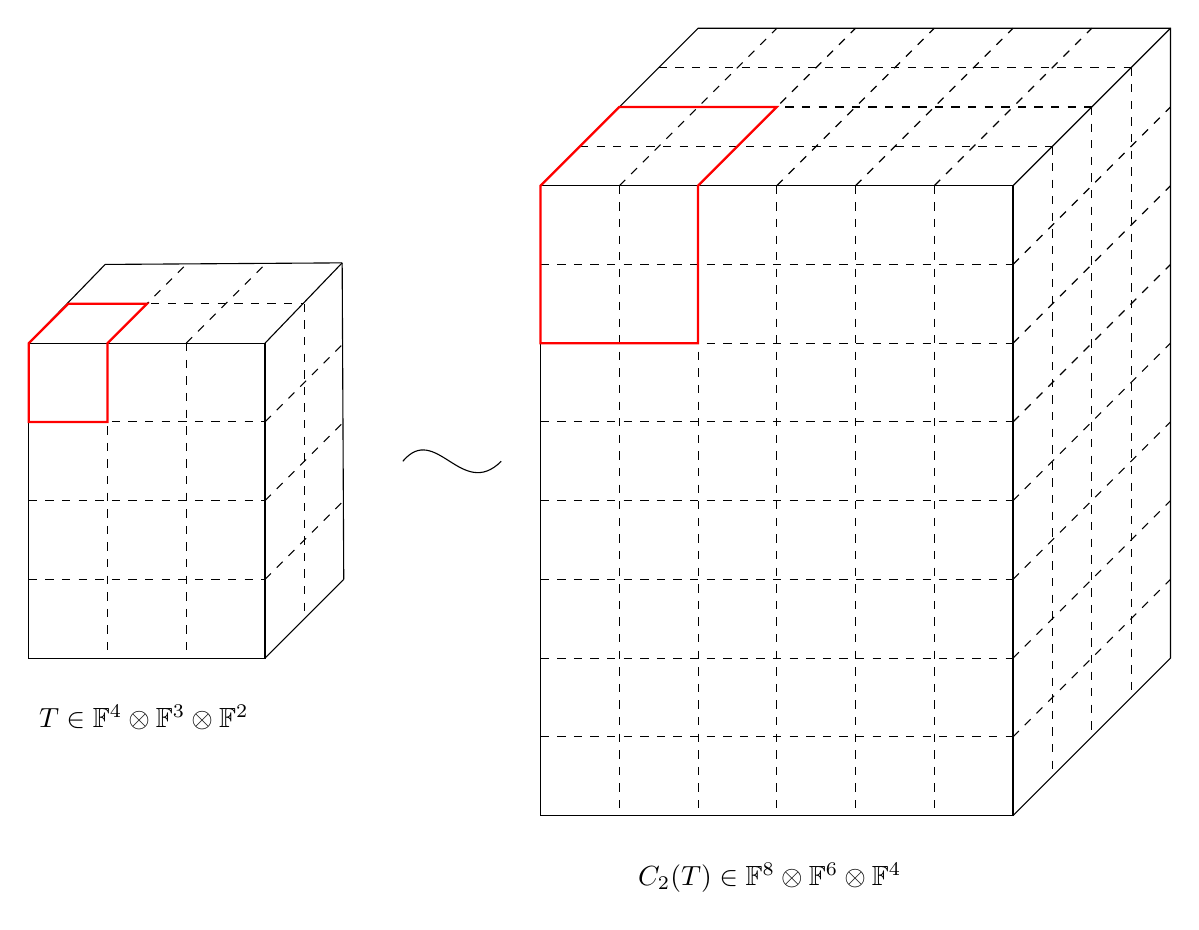
\begin{tikzpicture}[scale=1]
        % Coordinates
        \coordinate (A) at (1.00, 8.00);
        \coordinate (B) at (1.97, 9.00);
        \coordinate (C) at (4.00, 8.00);
        \coordinate (D) at (4.98, 9.02);
        \coordinate (E) at (4.00, 4.00);
        \coordinate (F) at (5.00, 5.00);
        \coordinate (G) at (1.50, 8.50);
        \coordinate (H) at (4.50, 8.50);
        \coordinate (I) at (4.50, 4.50);
        \coordinate (J) at (2.00, 8.00);
        \coordinate (K) at (2.00, 4.00);
        \coordinate (L) at (3.00, 8.00);
        \coordinate (M) at (3.00, 4.00);
        \coordinate (N) at (3.00, 9.00);
        \coordinate (O) at (4.00, 9.00);
        \coordinate (P) at (1.00, 7.00);
        \coordinate (Q) at (4.00, 7.00);
        \coordinate (R) at (5.00, 8.00);
        \coordinate (S) at (1.00, 6.00);
        \coordinate (T) at (4.00, 6.00);
        \coordinate (U) at (5.00, 7.00);
        \coordinate (V) at (1.00, 5.00);
        \coordinate (W) at (4.00, 5.00);
        \coordinate (X) at (5.00, 6.00);
        \coordinate (Y) at (7.50, 10.00);
        \coordinate (Z) at (9.50, 12.00);
        \coordinate (AA) at (15.50, 12.00);
        \coordinate (AB) at (15.50, 4.00);
        \coordinate (AC) at (13.50, 2.00);
        \coordinate (AD) at (13.50, 10.00);
        \coordinate (AE) at (8.50, 10.00);
        \coordinate (AF) at (10.50, 12.00);
        \coordinate (AG) at (9.50, 10.00);
        \coordinate (AH) at (11.50, 12.00);
        \coordinate (AI) at (10.50, 10.00);
        \coordinate (AJ) at (12.50, 12.00);
        \coordinate (AK) at (11.50, 10.00);
        \coordinate (AL) at (13.50, 12.00);
        \coordinate (AM) at (12.50, 10.00);
        \coordinate (AN) at (14.50, 12.00);
        \coordinate (AO) at (8.50, 2.00);
        \coordinate (AP) at (9.50, 2.00);
        \coordinate (AQ) at (10.50, 2.00);
        \coordinate (AR) at (11.50, 2.00);
        \coordinate (AS) at (12.50, 2.00);
        \coordinate (AT) at (8.00, 10.50);
        \coordinate (AU) at (14.00, 10.50);
        \coordinate (AV) at (8.50, 11.00);
        \coordinate (AW) at (14.50, 11.00);
        \coordinate (AX) at (9.00, 11.50);
        \coordinate (AY) at (15.00, 11.50);
        \coordinate (AZ) at (7.50, 9.00);
        \coordinate (BA) at (13.50, 9.00);
        \coordinate (BB) at (7.50, 8.00);
        \coordinate (BC) at (13.50, 8.00);
        \coordinate (BD) at (7.50, 7.00);
        \coordinate (BE) at (13.50, 7.00);
        \coordinate (BF) at (7.50, 6.00);
        \coordinate (BG) at (13.50, 6.00);
        \coordinate (BH) at (7.50, 5.00);
        \coordinate (BI) at (13.50, 5.00);
        \coordinate (BJ) at (7.50, 4.00);
        \coordinate (BK) at (13.50, 4.00);
        \coordinate (BL) at (7.50, 3.00);
        \coordinate (BM) at (13.50, 3.00);
        \coordinate (BN) at (15.50, 11.00);
        \coordinate (BO) at (15.50, 10.00);
        \coordinate (BP) at (15.50, 9.00);
        \coordinate (BQ) at (15.50, 8.00);
        \coordinate (BR) at (15.50, 7.00);
        \coordinate (BS) at (15.50, 6.00);
        \coordinate (BT) at (15.50, 5.00);
        \coordinate (BU) at (14.00, 2.50);
        \coordinate (BV) at (14.50, 3.00);
        \coordinate (BW) at (15.00, 3.50);
        \coordinate (BX) at (2.00, 7.00);
        \coordinate (BY) at (2.50, 8.50);
        \coordinate (BZ) at (9.50, 8.00);
        \coordinate (CA) at (10.50, 11.00);
        \coordinate (CB) at (5.75, 6.50);
        \coordinate (CC) at (7.00, 6.50);
        \coordinate (CD) at (6.17, 7.00);
        \coordinate (CE) at (6.50, 6.00);
        \coordinate (CF) at (2.46, 2.97);
        \coordinate (CG) at (10.41, 0.90);

        % Drawing
        \draw (1,4) rectangle (4,8);
        \draw (A) -- (B);
        \draw (C) -- (D);
        \draw (E) -- (F);
        \draw (B) -- (D);
        \draw (F) -- (D);
        \draw[dashed] (G) -- (H);
        \draw[dashed] (H) -- (I);
        \draw[dashed] (J) -- (K);
        \draw[dashed] (L) -- (M);
        \draw[dashed] (J) -- (N);
        \draw[dashed] (L) -- (O);
        \draw[dashed] (P) -- (Q);
        \draw[dashed] (Q) -- (R);
        \draw[dashed] (S) -- (T);
        \draw[dashed] (T) -- (U);
        \draw[dashed] (V) -- (W);
        \draw[dashed] (W) -- (X);
        \draw (7.5,2) rectangle (13.5,10);
        \draw (Y) -- (Z) -- (AA) -- (AB) -- (AC);
        \draw (AD) -- (AA);
        \draw[dashed] (AE) -- (AF);
        \draw[dashed] (AG) -- (AH);
        \draw[dashed] (AI) -- (AJ);
        \draw[dashed] (AK) -- (AL);
        \draw[dashed] (AM) -- (AN);
        \draw[dashed] (AE) -- (AO);
        \draw[dashed] (AG) -- (AP);
        \draw[dashed] (AI) -- (AQ);
        \draw[dashed] (AK) -- (AR);
        \draw[dashed] (AM) -- (AS);
        \draw[dashed] (AT) -- (AU);
        \draw[dashed] (AV) -- (AW);
        \draw[dashed] (AX) -- (AY);
        \draw[dashed] (AZ) -- (BA);
        \draw[dashed] (BB) -- (BC);
        \draw[dashed] (BD) -- (BE);
        \draw[dashed] (BF) -- (BG);
        \draw[dashed] (BH) -- (BI);
        \draw[dashed] (BJ) -- (BK);
        \draw[dashed] (BL) -- (BM);
        \draw[dashed] (BA) -- (BN);
        \draw[dashed] (BC) -- (BO);
        \draw[dashed] (BE) -- (BP);
        \draw[dashed] (BG) -- (BQ);
        \draw[dashed] (BI) -- (BR);
        \draw[dashed] (BK) -- (BS);
        \draw[dashed] (BM) -- (BT);
        \draw[dashed] (AU) -- (BU);
        \draw[dashed] (AW) -- (BV);
        \draw[dashed] (AY) -- (BW);
        \draw[red, thick] (P) -- (BX) -- (J) -- (BY) -- (G) -- (A) -- cycle;
        \draw[red, thick] (Y) -- (BB) -- (BZ) -- (AG) -- (CA) -- (AV) -- cycle;
        \draw (CB) .. controls (6.17, 7.00) and (6.50, 6.00) .. (CC);
        \node[above] at (CF) {$T \in \mathbb{F}^4\otimes\mathbb{F}^3\otimes\mathbb{F}^2$};
        \node[above] at (CG) {$C_2(T) \in \mathbb{F}^8\otimes\mathbb{F}^6\otimes\mathbb{F}^4
        $};
    \end{tikzpicture}
    \caption{$2$ clone of a tensor $T$}\label{figure:cloningtensor}
\end{figure}
\section{Seigals Counterexample over $\reals$}\label{section:seigalcounterexample}
\subsection{Details of Construction}\label{subsection:seigaldetails}
\subsection{Emulating Family Construction}\label{subsection:emulatingfamily}
\chapter{Conclusion}\label{chapter:conclusion}
\section{Further Work}\label{section:furtherwork}
\printbibliography

\newpage
% ----------------------- Back cover ------------------------------
% Please fill in:
% - Department
% - Department's address
% - Telephone number and fax number
% -----------------------------------------------------------------
\thispagestyle{empty}
\sffamily
%
\begin{textblock}{191}(113,-11)
{\color{blueline}\rule{160pt}{5.5pt}}
\end{textblock}
%
\begin{textblock}{191}(168,-11)
{\color{blueline}\rule{5.5pt}{59pt}}
\end{textblock}
%
\begin{textblock}{183}(-24,-11)
\textblockcolour{}
\flushright
\fontsize{7}{7.5}\selectfont
\textbf{Department of Mathematics}\\
Celestijnenlaan 200B\\
3001 LEUVEN (HEVERLEE), BELGI\"{E}\\
tel. + 32 16 32 70 07\\
fax + 32 16 32 79 98\\
wis.kuleuven.be\\
\end{textblock}
%
\begin{textblock}{191}(154,-7)
\textblockcolour{}
\includegraphics*[height=16.5truemm]{sedes}
\end{textblock}
%
\begin{textblock}{191}(-20,235)
{\color{bluetitle}\rule{544pt}{55pt}}
\end{textblock}
\end{document}
